%!TEX root = ../lections.tex

Рассмотрим в качестве осциллятора обычный маятник, совершающий малые колебания около нижней точки равновесия. Пусть у нас есть система из связанных осцилляторов (см. рис. \ref{fig:1}): маятники с точками подвеса на расстоянии $a$ друг от друга, связанные пружинками жесткости $\gamma$. 

\begin{figure}[h!]
	\centering
	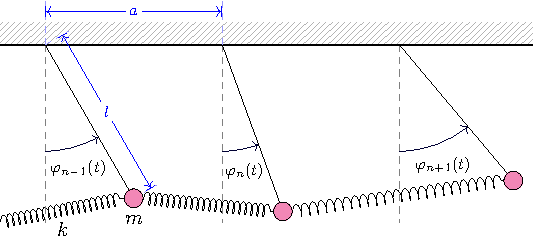
\includegraphics[scale=1.5]{img/osci_and_wave_in_ordered_struct/struct_of_pend}
	\label{fig:fig1}
\end{figure}

Обозначим $n$ -- номер маятника, $\omega_0^2=\frac{g}{l}$ -- собственная частота. Угол отклонения $n$-го маятника $\phi_n$, причем мы рассматриваем случай малых углов.


Состояние маятника зависит не только от времени $t$, но и от номера маятника $n$, то есть $n$ в некотором смысле играет роль пространственной координаты. Запишем уравнение динамики такого маятника:

\begin{equation}
	\ddot{\phi}_n+\omega^2_o \phi_n=\frac{\gamma}{m}\qty[\vphantom{\bigg|}(\phi_{n-1}-\phi_n)+(\phi_{n+1}-\phi_n)].
	\label{eq:1}
\end{equation}

Каждый маятник действует на соседние, причём сила взаимодействия зависит от разности значений углов. Упростим уравнение \eqref{eq:1}:

\begin{equation*}
	\ddot{\phi}_n+\omega^2_o \phi_n=\frac{\gamma}{m}\qty[\vphantom{\bigg|}\phi_{n-1}-2\phi_n+\phi_{n+1}].
\end{equation*}

Часто такую связь называют диффузионной, хотя, конечно, никакого отношения к процессу диффузии она не имеет. В системе нет диссипации, она линейна (нелинейность порождала бы новые частоты). Поэтому решение будем искать в следующем виде:
\begin{equation}
	\phi_n=A e^{i(\omega t-nka)}.
	\label{eq:2}
\end{equation}

Такая форма записи учитывает, что возмущение от маятника к маятнику проходит за некоторое конечное время.
\begin{equation}
	-\omega^2+\omega_0^2=\frac{\gamma}{m}\qty(e^{-ika}-2+e^{ika})
	\quad \Rightarrow \quad
	\omega^2=\omega_0^2-\frac{\gamma}{m}\qty(e^{-ika}-2+e^{ika})
	\label{eq:3}
\end{equation}
Рассмотрим случай  действительного $k$. Тогда
\begin{equation}
	\omega^2=\omega_0^2-\frac{\gamma}{m}(-2+2\cos{ka})=\omega_0^2+\frac{4\gamma}{m}\sin^2{\frac{ka}{2}}.
	\label{eq:4}
\end{equation}
Итак, мы установили, что $\omega$ и $k$ связаны соотношением \eqref{eq:4}. Построим график $\omega(k)$:
\begin{figure}[H]
	\centering
	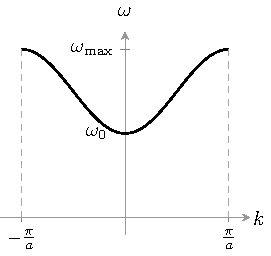
\includegraphics[scale=1.5]{img/osci_and_wave_in_ordered_struct/disp_of_struct}
\end{figure}
Нетрудно получить из уравнения \eqref{eq:4}, что 
\begin{equation*}
	\omega_{\max}=\sqrt{\omega_0^2+\frac{4\gamma}{m}}.
\end{equation*}
Если $\omega_0 < \omega < \omega_{max}$, то каждому $\omega$ соответствуют действительные $k_0$ и $-k_0$. Это означает, что каждой частоте соответствует две гармонические бегущие волны
\begin{equation*}
	\phi_n=A e^{i(\omega t+nk_0a)} 
	\qquad\text{и}\qquad
	\phi_n=A e^{i(\omega t-nk_0a)},
\end{equation*}
где $k_0$ -- волновое число. Поскольку система линейна, любая линейная комбинация решений тоже будет решением. 

Диапазон $\omega_0 < \omega < \omega_{\max}$ называют \textbf{полосой прозрачности} или полосой пропускания. Вне этой полосы решению не отвечают действительные $k$. В этом случае число \textit{$k$ - чисто мнимое} (чисто -- так как нет диссипации в системе) и $k=i\kappa$. Подставив такую связь в \eqref{eq:4}, получим
\begin{equation}
	\omega^2=\omega_0^2-\frac{4\gamma}{m}\sh^2{\frac{\varkappa a}{2}}.
	\label{eq:5}
\end{equation}
Подставляя \eqref{eq:5} в \eqref{eq:2}, получим вид волны в этом случае $\phi_n=A e^{-n\varkappa a} e^{i\omega t}$. Заметим, что при $n\rightarrow \infty$ функция  $\phi_n \rightarrow 0$, то есть в этих областях волна не проходит. 

Если мы находимся в полосе прозрачности, то $v_\text{фаз}=v_\text{фаз}(k), v_\text{фаз}=v_\text{фаз}(\omega)$. Если фазовая скорость зависит от частоты или волнового числа, то среда диспергирующая, а \eqref{eq:4} - дисперсионное соотношение. 

Дисперсия возникает из-за наличия собственных пространственных и временных масштабов : $a$ и $\omega_0$. У каждой компоненты волнового пакета будет своя фазовая скорость, возникнет его деформация. Именно наличием собственных масштабов объясняется то, что в одних случаях система пропускает волну, а в других нет.





\subsection{Предельный переход от цепочной структуры к среде}
Введем пространственную координату $x$ вдоль балки. Сделаем замену, считая, что $\phi_n$ зависит от двух переменных:
\begin{gather*}
	\phi_n(t) \rightarrow \phi(x,t), \\
	\phi_{n+1}(t) \rightarrow \phi(x+a,t)=\phi(x,t)+\pdv{\phi}{x}a +\frac12 \pdv[2]{\phi}{x}a^2+\dots
\end{gather*}

Считая a малым, разложим в ряд по степеням a:

\begin{equation}
	\phi_{n-1}(t) \rightarrow \phi(x-a,t)=\phi(x,t)-\pdv{\phi}{x}a +\frac12 \pdv[2]{\phi}{x}a^2+\dots,
	\label{eq:6}
\end{equation}
и подставим в \eqref{eq:1}

\begin{gather*}
	\pdv[2]{\phi}{t} + \omega_0^2 \phi=\frac{\gamma}{m}a^2 \pdv[2]{\phi}{x}, \\
	\frac{\gamma}{m}a^2 = v^2,
\end{gather*}
\begin{equation}
	\pdv[2]{\phi}{t}-v^2\pdv[2]{\phi}{x}+\omega_0^2\phi=0 -\text{Уравнение Клейна-Гордона}.
	\label{eq:7}
\end{equation}

Уравнение \eqref{eq:7} не что иное, как уравнение в частных производных. Когда мы можем использовать \eqref{eq:7} вместо \eqref{eq:1}?

Предполагали, что
\begin{enumerate}
	\item $\phi_n$, определенная в точке, определена и между дискретными точками подвеса;
	\item отброшены величины третьего порядка;
	\item a-мало
\end{enumerate}

Построим дисперсионную характеристику для \eqref{eq:7}

\begin{gather*}
	\phi(x,t)=Ae^{i(\omega t + kx)}, \\ -\omega^2-k^2v^2+\omega_0^2=0,
\end{gather*}
\begin{equation}
	\omega^2 = \omega_0^2 + k^2v^2.
	\label{eq:8}
\end{equation}
\begin{figure}[H]
	\centering
	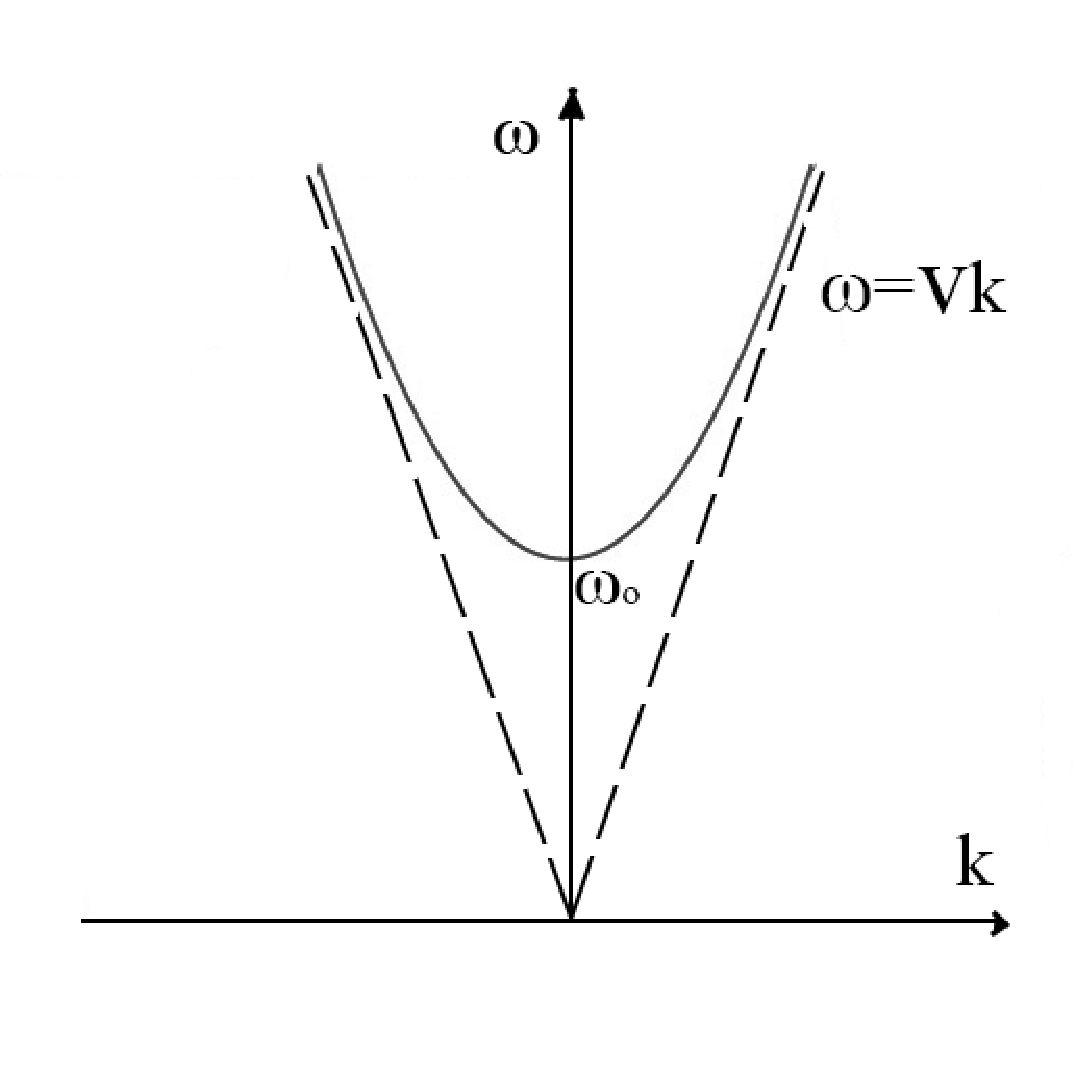
\includegraphics[width=0.5\linewidth]{fig/fig3.pdf}   
\end{figure}

Есть две асимптоты. 

При каких условиях дисперсионки совпадут?

$\lambda\gg a$ или $ka\ll$ - условие длинноволновой зоны, можно от одной перейти к другой, поскольку пространственный масштаб не сказывается, мы им пренебрегаем. Если $\omega_0 \rightarrow 0$, то из \eqref{eq:8}: $\omega^2=k^2v^2$. В этом случае система не обладает дисперсией. 

\begin{figure}[H]
	\centering
	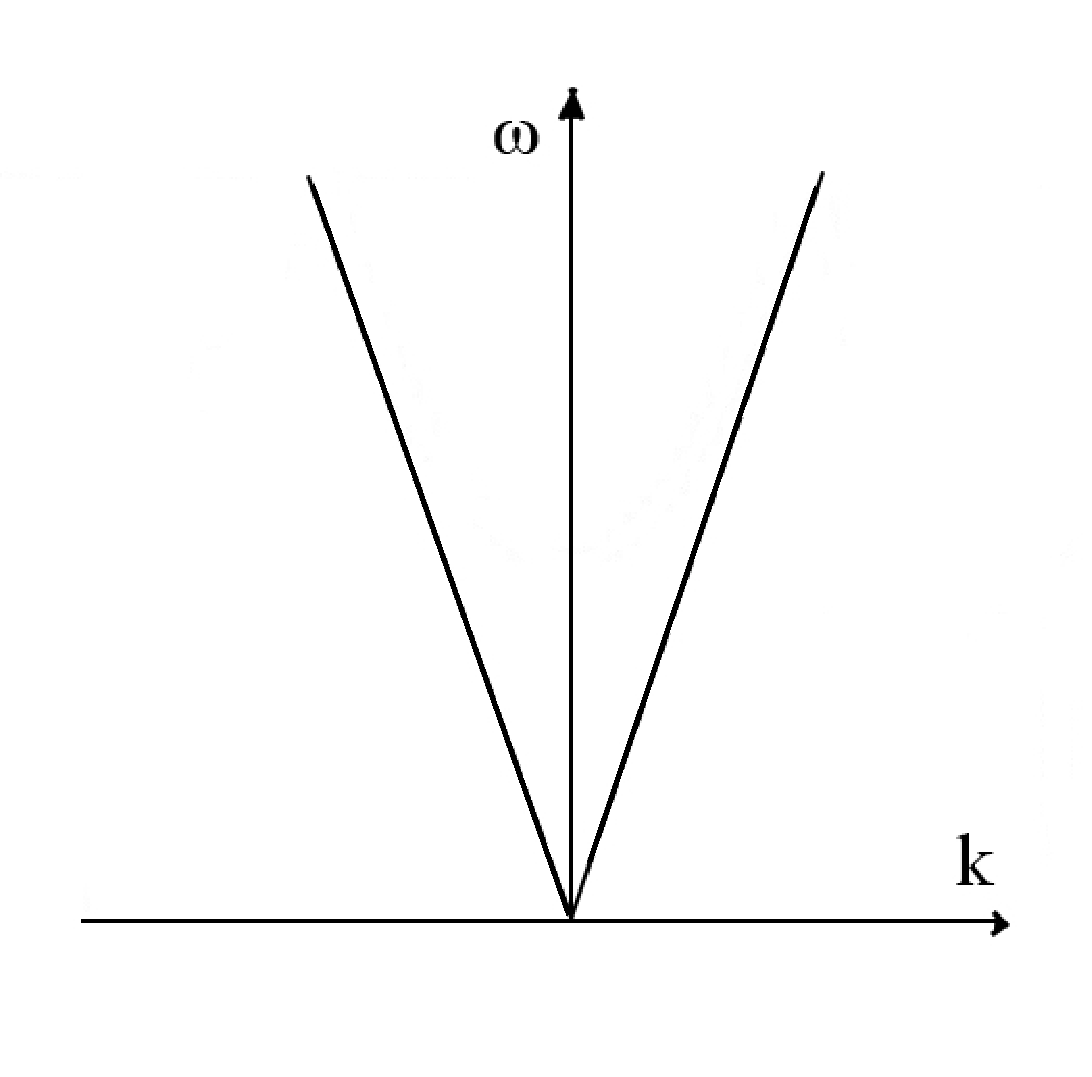
\includegraphics[width=0.5\linewidth]{fig/fig4.pdf}   
\end{figure}

Дисперсионная характеристика проявляется в области прозрачности/непрозрачности и зависимости $v_\text{фаз}$ от k или $\omega$.

Получили, шарики плотно друг к другу и покоятся.

Переход от цепочки к среде называется длинноволновым переходом. при нем теряется дискретность системы.

\subsection{Составление дисперсионного уравнения для произвольной линейной системы}

Рассмотрим многомерную систему
\begin{equation}
	A\pdv{\vec{U}}{t}+B\pdv{\vec{U}}{x}+C\vec{U}=0.
	\label{eq:9}
\end{equation}

A, B, C - $n\times n$ - матрицы; $\vec{U}(x,t)$ описывает состояние системы.

\begin{equation}
	\vec{U}=\vec{\phi} e^{i(\omega t - kx)}.
	\label{eq:10}
\end{equation}

\begin{equation*}
	\vec\phi=
	\begin{pmatrix}
		\phi_1 \\
		\phi_2 \\
		\phi_3 \\
		\vdots \\
		\phi_n \\
	\end{pmatrix}
	,
\end{equation*}

\begin{equation*}
	Ai\omega\vec\phi-iBk\vec\phi+C\vec\phi=0,
\end{equation*}
\begin{equation}
	(A\omega-Bk-iC)\vec\phi i=0.
	\label{eq:11}
\end{equation}

\eqref{eq:11} представляет собой систему линейных однородных уравнений относительно компонент вектора $\vec\phi$. Она имеет решение, если ее детерминант
\begin{equation}
	det(A\omega-Bk-iC)=0.
	\label{eq:12}
\end{equation}

для краткости обозначают $D(\omega,k)=0$. он связывает $\omega$ и k, т.е. задает дисперсионную характеристику. Следовательно, для $\forall k$ дисперсионное соотношение определяют n значений $\omega$: $\omega_1(k), \dots, \omega_n(k)$. Каждой паре k, $\omega_s(k)$ отвечает некоторый вектор, определяемый \eqref{eq:11}. При этом решением будут не только $k, \omega, \vec\phi$, но и $k^*, \omega^*, \vec\phi^*$. Можно построить действительное решение:
\begin{equation}
	\vec{U}(x,t)=\vec\phi e^{i(\omega t-kx)}+\vec\phi^* e^{-i(\omega^* t-k^*x)}.
	\label{eq:13}
\end{equation}

\eqref{eq:13} задает гармоническую волну, если $k, \omega$ действительные. Если же $k, \omega$ комплексные, то \eqref{eq:13} задает нарастающее или затухающее колебание. При этом общее решение может выть записано в виде 
\begin{equation*}
	\vec{U}(x,t)=\sum_{s=1}^{n} \phi^{(s)}e^{i(\omega_s(k)t-kx)} + \text{к.с}.
\end{equation*}

Как только будут учтены граничные условия, получится аналог характеристического уравнения.

\subsection{Влияние граничных условий}
Предположим, маятники были свернуты в кольцо, следовательно, должно уложиться целое число полуволн: 

\begin{gather*}
	n=1,\dots,N;~~\phi_{n-1}-2\phi_n+\phi_{n+1}; \\
	k=\frac{2\pi n}{l};~~\phi_{N+1}=\phi_1;~~k=k_n.
\end{gather*}	

Примером распределенной системы может служить струна длины l, концы которой закреплены:
\begin{figure}[H]
	\centering
	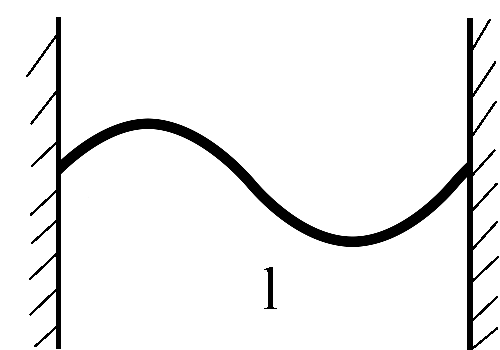
\includegraphics[width=0.5\linewidth]{fig/fig5.pdf}   
\end{figure}
\begin{gather*}
	U(x,t), \\ U(0,t)=u(l,t)=0, \\ U(x,t)=\phi_1 e^{i(\omega t-kx)}+\phi_2 e^{i(\omega t+kx)}, \\
	\begin{cases}
		\phi_1 e^{i\omega t}+\phi_2 e^{i\omega t}=0 \\
		\phi_1 e^{i\omega t}+\phi_2 e^{i\omega t+ikl}=0
	\end{cases}
	\\ \phi_1=-\phi_2,~~ \sin{kl}=0,~~ k=\frac{\pi n}{l}=k_n
\end{gather*}

\begin{equation}
	\begin{cases}
		D(\omega,k)=0 \\
		k=k_n
	\end{cases}
	\label{eq:14}
\end{equation}

Отсюда следует, что $\omega=omega_n$. Если среда без дисперсии, то спектры волновых чисел и волновых частот будут эквидистантными. 

\subsection{Устойчивость состояний равновесия нелинейных распределенных систем}
Простейшим типом решений распределенных систем являются такие состояния, которые не меняются ни во времени, ни в пространстве: $U(x,t); U=U_o=const$.
\begin{equation}
	\pdv{U}{t}=f(U)+D\pdv[2]{U}{x},
	\label{eq:15}
\end{equation}
где $f(U)$ - нелинейная функция. Пусть, кубическая. Если убрать D. то уравнение будет описывать динамику точки в среде.
\begin{figure}[H]
	\centering
	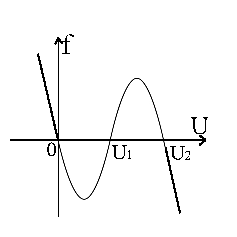
\includegraphics[width=0.5\linewidth]{fig/fig6.pdf}   
\end{figure}

Три точки, где $f(U)=0$. В системе могут быть стационарные решения (не зависящие от времени) - это другой тип решения. Будем рассматривать их решение в классе гармонических функций. 
\begin{equation*}
	\xi(x,t) \sim e^{pt+ikx}
\end{equation*}

Линеаризуем \eqref{eq:15} на состояниях равновесия:
\begin{equation*}
	U=U^*+\xi(x,t),
\end{equation*}
\begin{equation}
	\pdv{\xi}{t}=D\pdv[2]{\xi}{x}+f'(U^*)\xi(x,t).
	\label{eq:16}
\end{equation}
\begin{gather*}
	f(U^*+\xi(x,t))\approx f(U^*)+f'(U^*)\cdot\xi(x,t), \\ \xi(x,t)=A e^{pt+ikx} \\
	p =-Dk^2+f'(U^*), \\ U=0,~~U=U_2,~~f'(U^*)<0.
\end{gather*}

Для каждого А.
\begin{figure}[H]
	\centering
	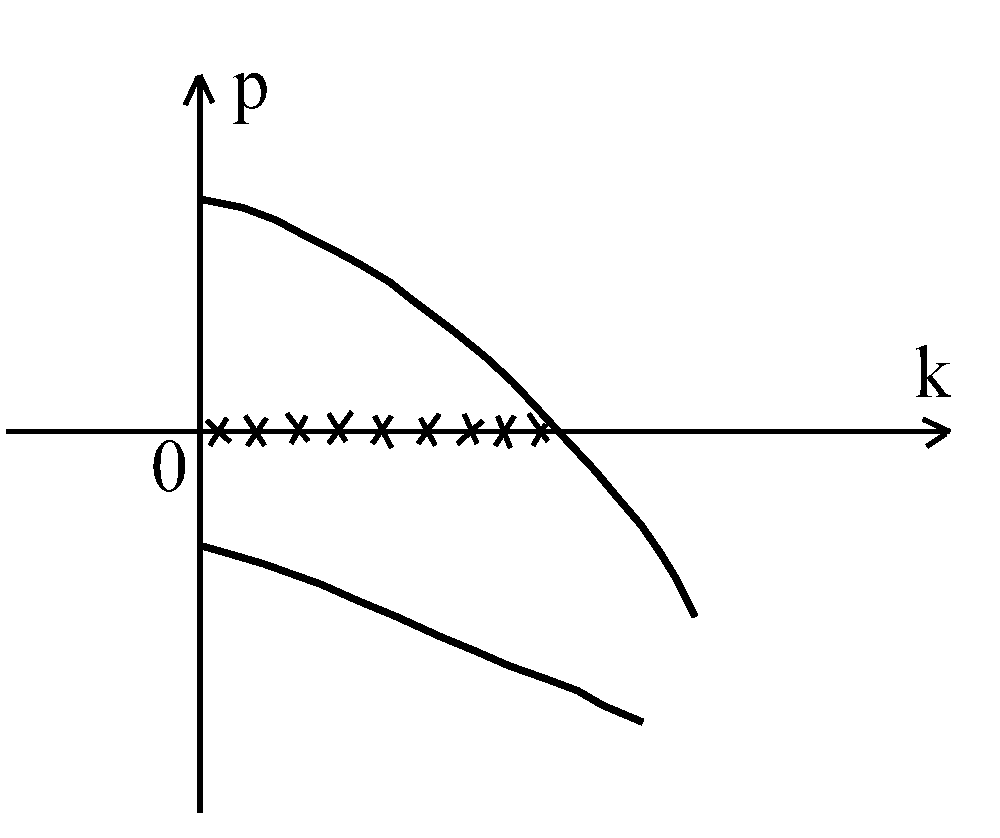
\includegraphics[width=0.5\linewidth]{fig/fig7.pdf}   
\end{figure}

Все решения такого вида затухают, следовательно, $U=0, U=U_2$ устойчивые, а $U_1$ - неустойчивое в классе возмущений $\xi(x,t)=A e^{pt+ikx}$.

В частности, \eqref{eq:15}, описывает распространение пламени по бикфордовому (огнепроводному) шнуру. Волна превращает вещество из несгоревшего материала в сгоревшее.
